\chapter{Databáze}

V této práci jsme využívali dvě databáze fotopletysmografických signálů: CapnoBase a BUT PPG.

Na těchto databázích jsme testovali a porovnávali výsledky použitých algoritmů.
U databáze CapnoBase jsme porovnávali naměřené systolické vrcholy s referenčními hodnotami a díky tomu jsme porovnávali i rozdíl v srdeční tepové frekvenci.
U databáze BUT PPG nebyly referenční hodnoty systolických vrcholů k dispozici, ale byly zde referenční hodnoty tepové frekvence signálů.

% ----------------------------------------------------------------------- %
\section{CapnoBase}

CapnoBase je databáze, která obsahuje signály získané během čtyřiceti dvou různých, klinických, situací.
V databázi jsou 8 minut dlouhé, elektrokardiografické, respirační a pro naši práci nejdůležitější, fotopletysmofrafické (PPG) signály.
Signály jsou vzorkovány při frekvenci 300 Hz a obsahují ručně označené referenční systolické vrcholy, což jsme využili pro vypočítání matice záměn [16].
Tyto vrcholy jsou označené podle záznamů elektrokardiogramů (EKG) [17].

% ----------------------------------------------------------------------- %
\section{BUT PPG}

\acl{BUT PPG} (\acs{BUT PPG}) je databáze vytvořená na Fakultě elektrotechniky a komunikačních technologií Vysokého učení technického v Brně.
Tato databáze byla vytvořena za účelem hodnocení kvality PPG signálů a odhadu srdeční frekvence (TF).
Data obsahují 48 desetisekundových záznamů PPG a souvisejících elektrokardiografických (EKG) signálů, které byly použity pro určení referenční TF.
Data byla shromážděna od 12 subjektů (6 žen a 6 mužů) ve věku od 21 do 61 let.
Záznamy byly provedeny mezi srpnem 2020 a říjnem 2020 pomocí smartphonu Xiaomi Mi9 se vzorkovací frekvencí 30 Hz [14].

Určení kvality PPG signálů bylo stanoveno pěti experty.
Tito experti určili TF pouze ze signálu PPG a výsledek porovnali s referenční TF vypočítané z EKG signálů.
Během hodnocení měli přístup k softwaru, který využíval techniky stacionární vlnkové transformace.
Využití tohoto programu bylo dobrovolné [22].

Jak bylo řečeno, data z BUT PPG byla nasnímána telefonem.
V této podkapitole tedy popíšeme postup, jak extrahovat PPG signál z videa.
Pro měření potřebujeme pouze kameru v mobilním telefonu a zapnutý blesk. 

Při sběru dat pro Brněnskou databázi přiložil subjekt ukazováček na fotoaparát tak, aby překrýval objektiv a LED svítilnu.
Při snímání vyzařuje LED světlo. Rozlišení videa bylo nastaveno na 720 x 1280 px a snímkovací frekvence na 30 Hz [2]. 

Z videa byl extrahován průměr červené složky, který sloužil jako surový PPG signál.
Jelikož fotoaparát pracuje se světlem odraženým, surový signál byl invertován.
Postup je zobrazen na obrázku \ref{fig:videoZaznamPPG}.

\begin{figure}[h]
	\centering
	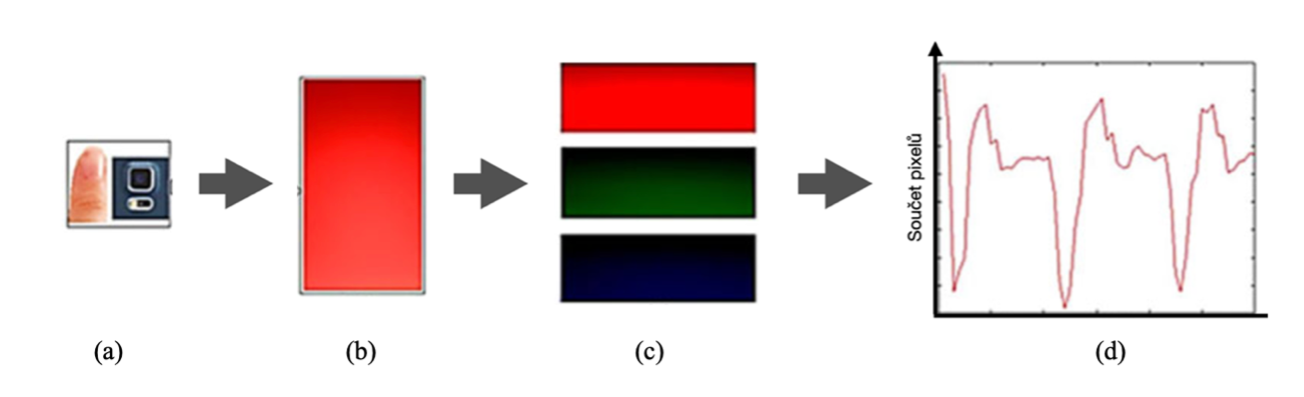
\includegraphics[width=0.8\textwidth]{./obrazky/videoZaznamPPG.png}
	\caption{Záznam videa na kameru mobilního telefonu (a), jeden vybraný snímek ze záznamu (b), snímek rozložen na tři barevné složky (c), PPG signál vykreslený z červené složky (d), upraveno z [6].}
	\label{fig:videoZaznamPPG}
\end{figure}
